\documentclass[11pt, a4paper]{article}
\usepackage[slovene]{babel}
\usepackage[T1]{fontenc}
\usepackage[utf8]{inputenc}
\usepackage{lmodern}
\usepackage{eurosym}
\usepackage{amssymb}
\usepackage{amsfonts}
\usepackage{amsmath}
\usepackage{graphicx}
\DeclareUnicodeCharacter{2212}{-}
\usepackage{graphicx}
\usepackage{subfig}
\usepackage{graphicx}
\graphicspath{ {images/} }


\renewcommand*\contentsname{Kazalo}

\pagenumbering{arabic}

\begin{document}

\begin{titlepage}

\begin{center}

\Huge 
\textbf{Skupina 22: \textsl{k}-means algoritem}

\vspace{1cm}
\Large
\textbf{Poročilo}

\vspace{1cm}
\large
Projekt v povezavi s predmetom Operacijske raziskave

\vspace{2,5cm}
\large
Avtorja:\\
\textbf{Matevž Raspet, Eva Šraj}\\

\vfill

\Large Ljubljana, november 2018

\end{center}
\end{titlepage}

\tableofcontents

\vspace{1 cm}

\listoffigures

\pagebreak

\section{KRATEK OPIS PROBLEMA}
\noindent Pri projektu iz predmeta Operacijskih raziskav bova preučevala delovanje \textsl{k}-means algoritma. 

\vspace{0,5cm}

\noindent \textbf{NAVODILO:} Zgeneriraj in predstavi naključne podatke v prostorih $\mathbb{R}$, $\mathbb{R}^2$ in $\mathbb{R}^3$, ki imajo strukturo množice in uporabi \textsl{k}-means algoritem s funkcijama oddaljenosti - \textbf{metoda Manhattan} in \textbf{metoda najmanjših kvadratov} (krajše MNK).
Preizkusi \textsl{k}-means algoritem na nizu podatkov, ki imajo 10\% bolj odstopajočih podatkov in primerjaj rezultate z uporabo obeh metod.
Za podatke, zgenerirane v  $\mathbb{R}^2$, poišči povezavo med \textsl{k}-means algoritmom z Vorionojevim diagramom in povezavo ponazori grafično. 

\subsection{Kaj je \textsl{k}-means algoritem in kako deluje?}

\noindent To je metoda vektorske kvantizacije, namenjena za analizo grupiranja podatkov, predvsem pri rudarjenju s podatki. Ta algoritem naredi particijo $n$ meritev v $k$ različnih množic, v katerih vsaka meritev pripada množici z najbližjo povprečno vrednostjo. Rezultat particije je razdelitev prostora v Voronojeve celice. \\
\noindent BOLJ FORMALNO: Naj bodo $(x_1, x_2, \ldots,x_n)$ dane meritve, kjer je vsaka meritev $x_i$ $d$-dimenzionalen realni vektor. \textsl{K}-means algoritem napravi particijo $n$ meritev v $k  (\leq n)$ množic $S= \{S_1, S_2, \ldots, S_k\}$, na podlagi najmanjše vsote kvadratov razdalj med meritvami posamezne množice in njihovim povprečjem $\mu_i$.

\vspace{0.5 cm}

\noindent Torej, s \textsl{k}-means algoritmom opravimo grupiranje $n$ naključnih podatkov v množice v treh korakih:
\begin{itemize}
	\item narišemo $k$ naključno izbranih točk v prostoru (prvotne vrednosti povprečnih vrednosti) $\mu_1^{(1)}, \dots, \mu_k^{(1)}$;
	\item v zadolžitvenem koraku (\textsl{angl. assignment step}), vsako točko določimo najbljižji povprečni vrednosti \\
$S_i^{(t)} = \{x_j:  \| x_j - \mu_i^{(t)} \|^2 \le  \| x_j - \mu_{i'}^{(t)} \|^2\ \forall  i' \in \{1, \ldots, k\} \}$
	\item v koraku nadgrajevanja (\textsl{angl. upgrade step}), zgeneriramo nove centroide množic
\begin{align*}
 \mu_i^{(t+1)} = \frac{1}{ | S_i^{(t)}| } \sum_{x_j \in S_i^{(t)}} x_j 
\end{align*}
\end{itemize}

\noindent Problem je sicer računsko zahteven, ker se ga ne da rešiti v polinomskem času (\textbf{NP-zahteven} algoritem). Vendar pa obstajajo učinkoviti hevristični algoritmi, ki se pogosto uporabljajo in se hitro približajo lokalnemu optimumu. 

\vspace{0,5cm}

\noindent Z najinim projektom sva se osredotočila predvsem na delovanje \textsl{k}-means algoritma in ga preizkusila na konkretnih podatkih v prostorih $\mathbb{R}$, $\mathbb{R}^2$ in $\mathbb{R}^3$.

\subsection{Neznani pojmi}

\noindent Kot sva omenila že zgoraj, sva uporabila 2 metodi za računanje razdalj - \textbf{metoda Manhattan} in \textbf{metoda najmanjših kvadratov} (krajše MNK).

\vspace{0.5 cm}

\noindent \textbf{Definicija:} Naj bosta $X$ in $Y$ $n$-razsežna vektorja; $X = (x_1, x_2, \ldots, x_n)$ in $Y = (y_1, y_2,\ldots, y_n).$ \\
Razdalja po \textbf{metodi Manhattan} je definirana kot: 
\begin{equation}
d(X, Y) = \sum_{i = 1}^n | x_i - y_i |
\end{equation}
Po \textbf{metodi najmanjših kvadratov} razdaljo definiramo kot:
\begin{equation}
d(X, Y) = \sqrt {\sum_{i = 1}^n (x_i - y_i)^2}
\end{equation}

\noindent \textsc{Voronojev diagram} \\

\noindent V matematiki Voronojev diagram prikazuje razdelitev ploskve na območja, osnovana na najmanjši razdalji točk do centra v posameznih množicah. Obarva nam podatke, ki spadajo k istemu centru. 

\vspace{0,5 cm}

\newpage

\section{PODATKI V PROSTORU $\mathbb{R}$}

\noindent \textbf{CILJ:} S pomočjo \textsl{k}-means algoritma sva na podlagi deleža posameznih krvnih skupin v izbranih evropskih državah določila tipe krvnih skupin. \\

\noindent Iz Wikipedije sva v program RStudio uvozila podatke o porazdelitvi krvnih skupin po državah. Zaradi boljše preglednosti na grafu in boljšega ujemanja podatkov sva se omejila le na evropske države. \\

\noindent \textbf{PODATKI:} \\
\noindent Za 37 izbranih evropskih držav sva uvozila deleže posameznih krvnih skupin v tabelo.
\noindent Za vsako državo sva pogledala porazdelitev na 8 krvnih skupin, imenovanih 0+, A+, B+, AB+, 0-, A-, B- in AB-.\\

\noindent Glede na formalno definicijo \textsl{k}-means algoritma so podatki: \\
\begin{itemize}
	\item $ x_1,…,x_{37}$, kjer $x_i$ prikazuje izbrano evropsko državo,\\
	\item $\forall x_i  (i = 1,\ldots, 37)$ je 8-dimanzionalni vektor $\Rightarrow$ v vsaki državi je 8 tipov krvnih skupin \\
\end{itemize}
 S \textsl{k}-means algoritmom sva napravila particijo 37 meritev v 8 množic, \\ $ S = \{S_1, \ldots, S_8\}$. \\
 Množice nisva poimenovala, ampak samo oštevilčila od 1 do 8. \\

\noindent \textbf{REZULTATI:} \\

\begin{figure}[h]
\caption{Graf MNK: Delež krvnih skupin v izbranih evropskih državah}
\centering
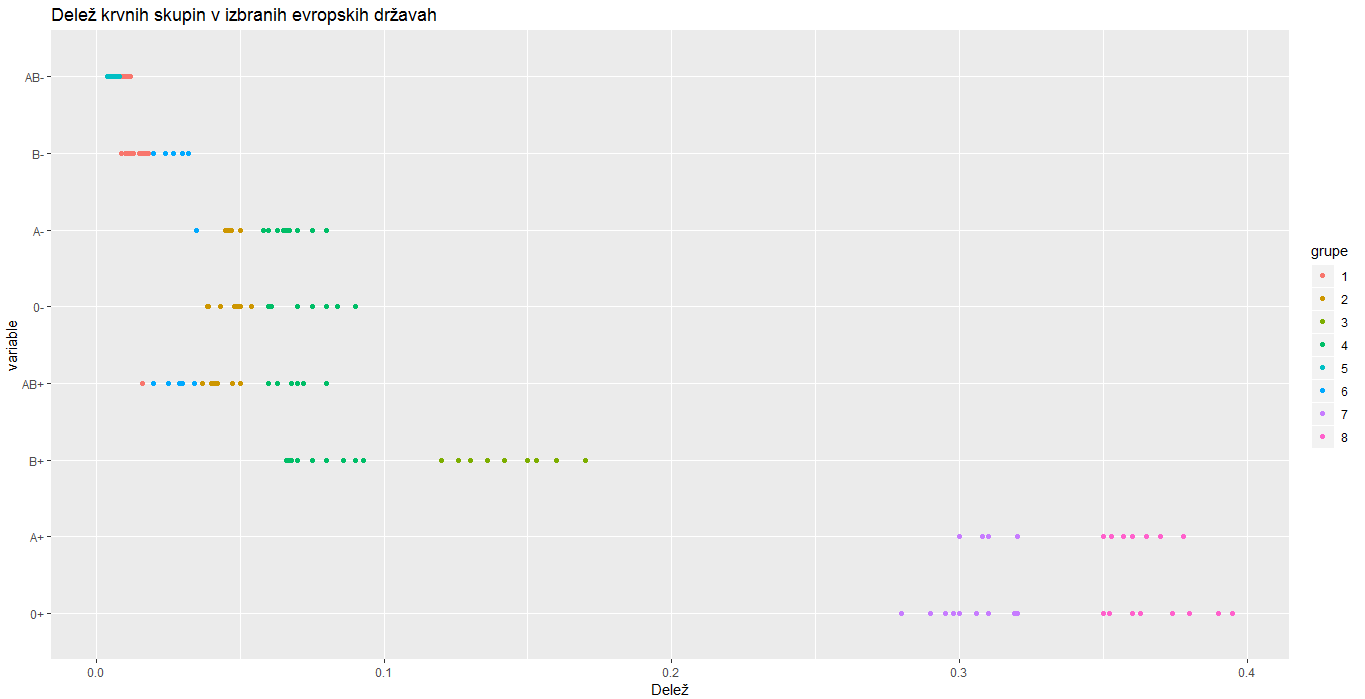
\includegraphics[width=12cm, height=6cm]{grafMNKkri}
\end{figure}

\noindent Kot je razvidno iz grafa zgoraj, se število krvnih skupin znotraj iste množice razlikuje. \\
V množici $S_1$ imamo samo krvno skupino AB-, medtem ko so v množici $S_5$ kar 4 (A-, 0-, AB+, B+). Po drugi strani pa ima množica $S_6$ samo krvno skupino B+, kar pomeni da sva v tej množici uspela pogrupirati samo podatke iz ene krvne skupine, B+.\\

\noindent Poskušala sva pogrupirati podatke na način, da bi bila v vsaki množici natanko ena krvna skupina, kar pa nama je uspelo le na množicah $S_1$ in $S_6$. V vseh ostalih pa so zastopani tipi večih različnih krvnih skupin, kar pa ni optimalno.

\vspace{0.5 cm}

\noindent Deleži krvnih skupin so med evropskimi državami podobno zastopane – najmanj ljudi ima krvno skupino AB-, najpogosteje pa sta zastopani krvni skupini 0+ in A+. 
\noindent Bolj gosto kot so narisane pikice na grafu, več držav ima podoben delež iste krvne skupne, takšna je krvna skupina AB-. Po drugi strani pa bolj poredko narisane pikice predstavljajo večja odstopanja deležev med državami znotraj posamezne krvne skupine. Kar je najbolj očitno pri krvni skupini 0+ (na Madržarskem in Češkem je delež le-te samo 0.27, v Islandija pa ta znaša 0.476 ).

\vspace{0.5 cm}

\noindent Glede na vse zgoraj opisano, je možno podatke še malo prečistiti.
\noindent Tako sva znotraj vsake množice z MNK poračunala oddaljenost posameznega podatka do centra. Te razdalje imajo vrednosti med $5.714\cdot10^{-6}$ (Velika Britanija, AB+) in $1.053\cdot10^{-1}$ (Irska, 0+).
Ker vrednosti bolj ali manj odstopajo od centra, sva 10\% najbolj odstopajočih izvzela. \\

\begin{figure}[h]
\caption{Graf Manhattan: Delež krvnih skupin v izbranih evropskih državah}
\centering
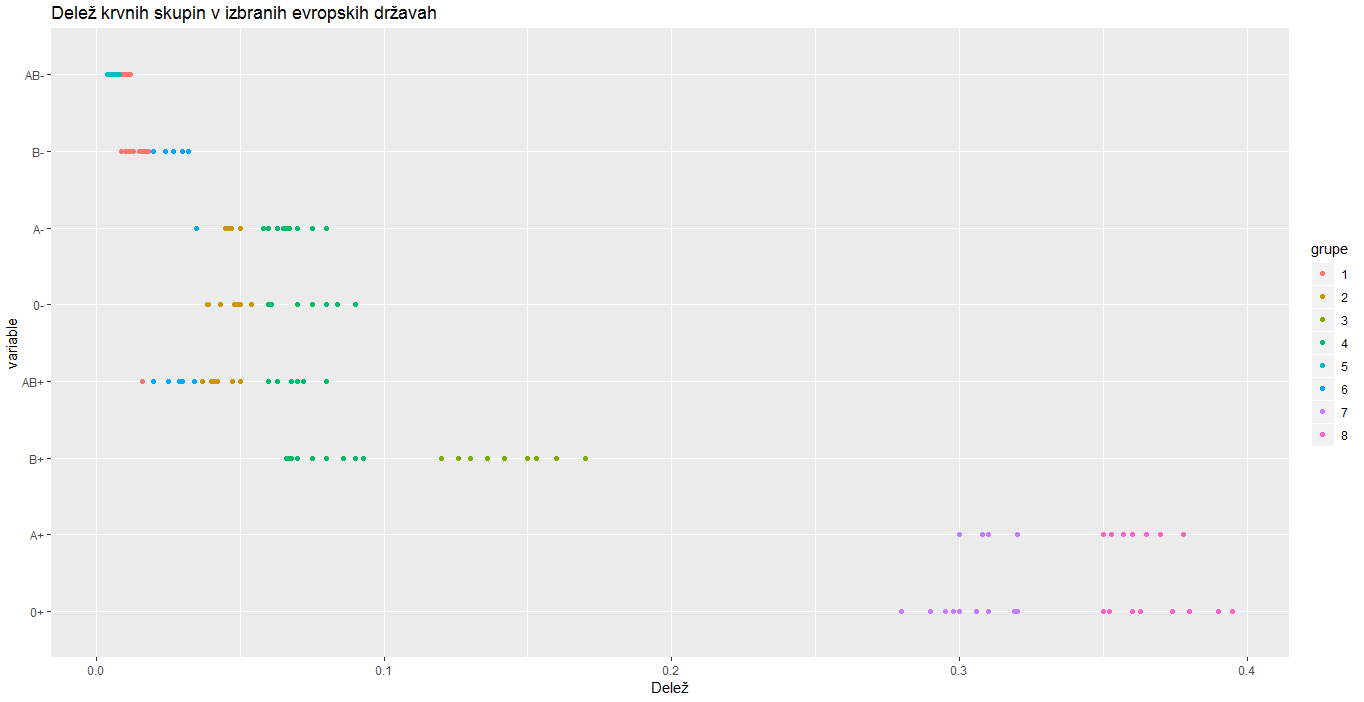
\includegraphics[width=12cm, height=6cm]{grafMNKoutkri}
\end{figure}

\noindent Zgornji graf predstavlja delež krvnih skupin evropskih držav, kjer sva izvzela 29 najbolj odstopajočih podatkov. Najbolj očitna razlika s prejšnjim grafom je zastopanost krvnih skupin A+ in 0+. To pa je povsem razumljivo, saj so pri teh 2 krvnih skupinah podatki najbolj razpršeni. \\

\noindent Poleg tega sva znotraj vsake množice poračunala tudi skupno vsoto razdalj podatkov do centrov, dobljeno po MNK. Razdalje pri množicah $S_1$ (temno modra barva), $S_2$ (rdeča barva), $S_5$ (temno zelena barva) in $S_6$ (svetlo zelena barva) so tudi po odstranitvi 10\% najbolj odstopajočih meritev ostale enake. Kar pomeni, da podatki od prej navedenih množic niso najbolj odstopali od centra. Medtem ko so se pri ostalih 4 množicah skupne razdalje znotraj iste množice očitno zmanjšale.

\vspace{0.5 cm}

\noindent Poleg metode MNK sva za računanje razdalj uporabila tudi metodo Manhattan. Poleg tega, sva narisala tudi grafa [graf.Manhattan] in \newline
[graf.Manhattan.outliers] (v datoteki prostorRkri.R), ki pa sta nama dala enake vrednosti in rezultate kot pri metodi MNK.

\vspace{0.5 cm}

\noindent TEORETIČNA UTEMELJITEV: V enačbah (1) in (2) sta neznanki:\\ 
$x_i$\ldots\ldots delež krvne skupine za vsako izbrano evropsko državo \\
$y_i$\ldots\ldots center posamezne množice, definirane s \textsl{k}-means algoritmom  \\
\begin{align*}
| x_i - y_i | = \sqrt{(x_i - y_i)^2}
\end{align*}

\newpage

\section{PODATKI V PROSTORU $\mathbb{R}^2$}
\subsection{PRIMER 1}
\noindent \textbf{CILJ:} S pomočjo \textsl{k}-means algoritma sva poskušala na podlagi statistike igralcev (zadeti goli in podeljene asistence), določiti igralne pozicije igralcev. \\

\noindent Iz spleta sva uvozila podatke o 100 svetovno znanih nogometaših.

\vspace{0.5 cm}

\noindent \textbf{PODATKI:} \\
\noindent Za vsakega igralca naju je zanimalo število zadetih golov in asistenc in na podlagi teh podatkov sva poskušala določiti igralne pozicije. \\

\noindent Za lažjo predstavo sva najprej narisala [graf1] (v datoteki prostorR2goli.R), ki prikazuje dejanske pozicije glede na statistiko. \\
\noindent Nato sva s pomočjo podatkov naredila grupiranje v tri skupine. Podatke sva poskušala pogrupirati glede na igralne pozicije tipov: 
\begin{itemize}
	\item napad: centre forward, second striker,
	\item sredina: attacking midfield, central midfield, left winger, right winger,
	\item obramba: centre back, defensive midfield, goalkeeper, right back, left back.
\end{itemize}

\noindent Glede na formalno definicijo \textsl{k}-means algoritma so podatki:
\begin{itemize}
	\item $x_1,\ldots,x_{100}$, kjer $x_i$ prikazuje posameznega nogometaša,
	\item $\forall x_i (i = 1,\ldots,100)$ je 2-dimanzionalni vektor $\Rightarrow$  prva komponenta prikazuje število asistenc posameznega igralca, druga komponenta pa število zadetih golov.\\
\end{itemize}
Z algoritmom sva napravila particijo 100 meritev v 3 množice, $S = \{S_1, S_2, S_3\}$, kjer $S_1$ predstavlja obrambo, $S_2$ sredino in $S_3$ napad.

\vspace{0.5 cm}

\noindent \textbf{REZULTATI:} \\

\begin{figure}[h]
\caption{Graf MNK: Izračun igralnih pozicij s pomočjo grupiranja}
\centering
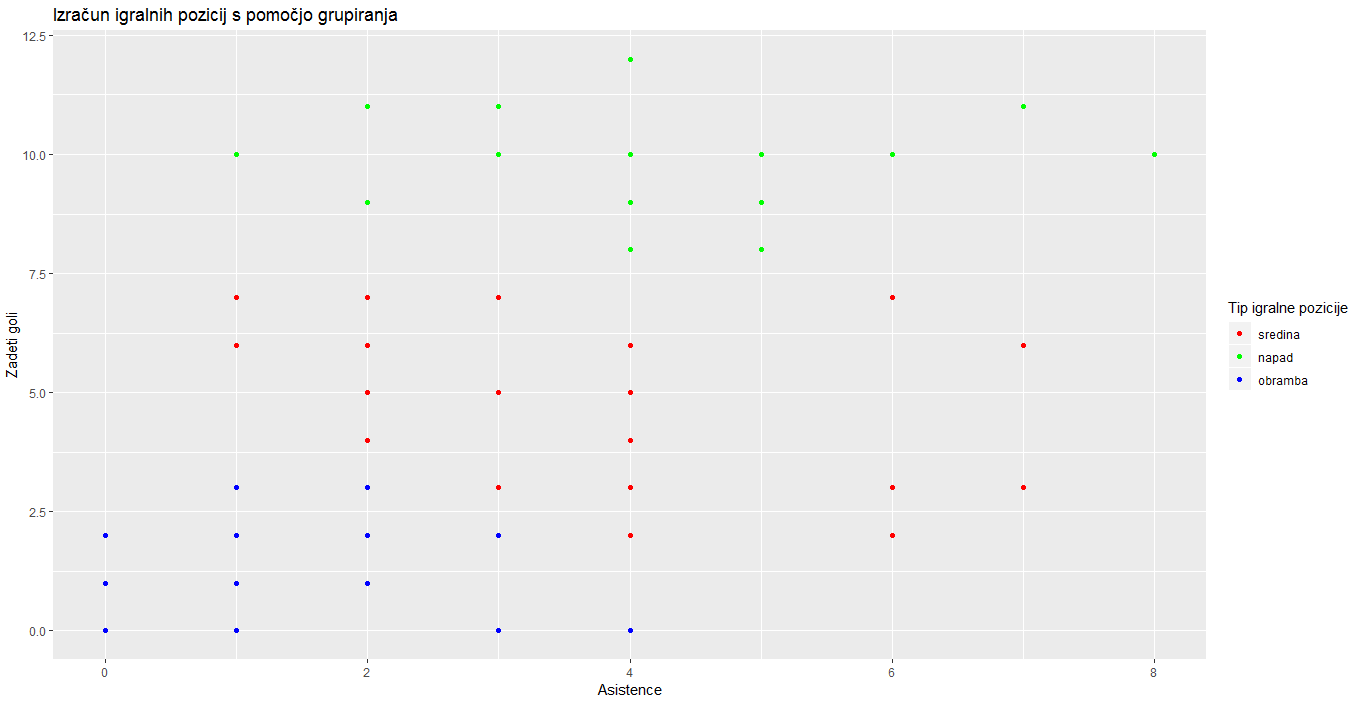
\includegraphics[width=12cm, height=6cm]{grafMNKoutgoli}
\end{figure}

\begin{figure}[h]
\caption{Graf MNK: Izračun igralnih pozicij s pomočjo grupiranja}
\centering
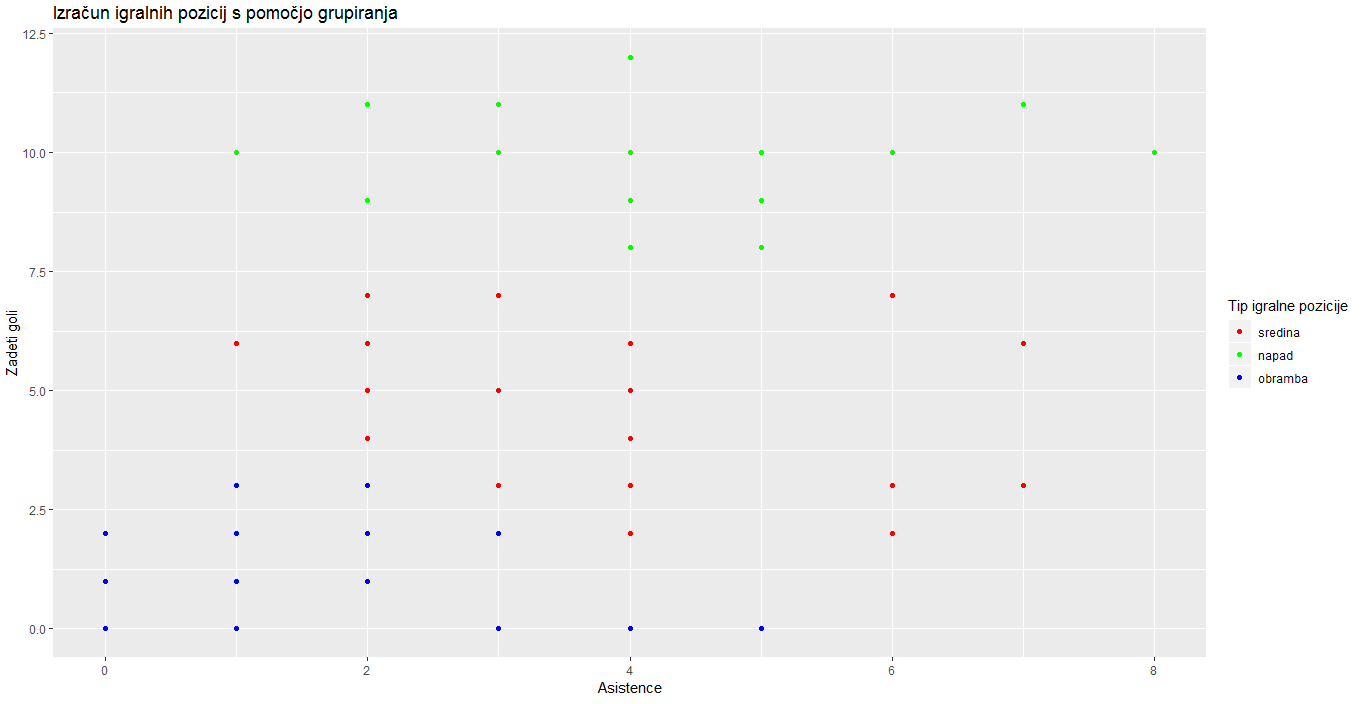
\includegraphics[width=12cm, height=6cm]{grafManhattanoutgoli}
\end{figure}

\noindent Iz dobljenih rezultatov in dejanskih igralnih pozicij lahko vidimo, da je \\
 \textsl{k}-means algoritem večinoma pravilno pogrupiral podatke v množice napad, sredina in obramba.\\
 V množici napad (modra barva) so najbolj zastopani podatki s pozicijami klasičnih napadalcev(\textsl{angl.centre forward}) in pa polnapadalec (\textsl{angl. second striker}), v množici sredina (zelena barva) igralci tipa centralnih veznih igralcev(\textsl{angl. central midfield}), v množici obramba (rdeča barva) pa vratarji \textsl({angl. goalkeeper}) in pa levi ter desni bočni igralci. \\
\noindent Prav tako sva s \textsl{k}-means algoritmom dobila povprečno število zadetih golov in asistenc po tipih igralnih pozicij napad, sredina in obramba. \\
\noindent Nekateri podatki so bili razvrščeni v napačne razrede, kar je bila posledica različnih dejavnikov. Predvsem so to napadalni igralci, ki niso izplonili svojih statistik zaradi poškodbe (niso zadevali, saj niso igrali vseh tekem), prav tako pa se je pojavil kakšen obrambni igralec (vendar redko), ki je izstopal iz svoje množice, saj je zadel več golov oziroma podelil več asistenc, kot se za igralca obrambne vrste pričakuje.

\vspace{0.5 cm}

\begin{figure}[h]
\caption{Voronojev diagram}
\centering
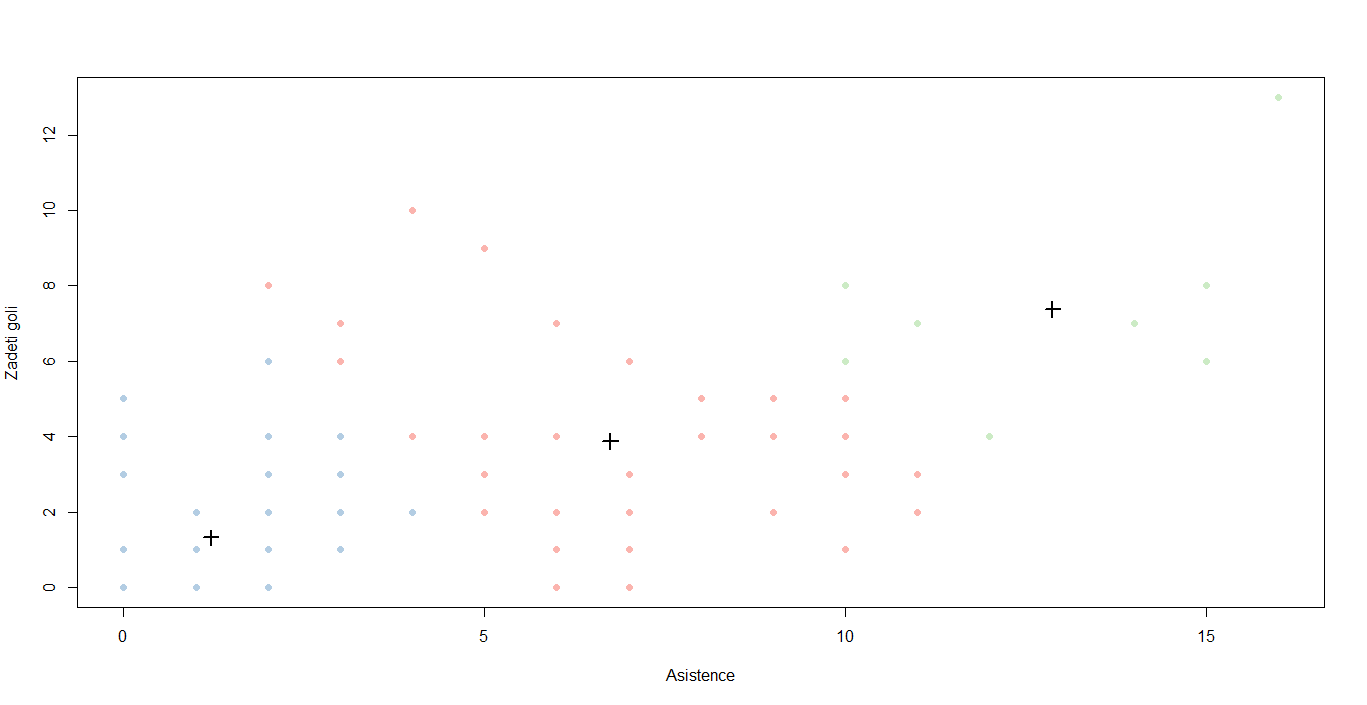
\includegraphics[width=12cm, height=6cm]{Voronojgoli}
\end{figure}

\noindent Prav tak opa sva za primer v $\mathbb{R}^2$ naredila Voronojev diagram.

\noindent Ta nama je razdelil območje na 3 različne dele. 

\subsection{PRIMER 2}
\textbf{CILJ:} Z algoritmom sva poskušala določiti kritična leta umrljivosti v Sloveniji v letu 2017. \\

\noindent Podatki, ki sva jih na spletu našla v obliki .csv, prikazujejo število umrlih ljudi po starostih.  

\vspace{0.5 cm}

\noindent \textbf{PODATKI:} \\
\noindent  Za vsako starost posebej (od 0 pa do 100+ let) sva pogledala število umrlih moških in žensk.  \\
\noindent V tabeli in na grafu sva zaradi večje preglednosti moške označila z 1 in ženske z 2. \\

\noindent Na začetku sva narisala [graf2] (v datoteki prostorR2umrli.R), kjer sva pogledla pogostost smrti za vsako starost, ločeno glede na spol. 
\noindent Nato sva s pomočjo \textsl{k}-means algoritma vse podatke pogrupirala v 3 množice glede na kritično starost. Te so:
\begin{itemize}
	\item najbolj - rdeča barva na grafu;
	\item srednje - modra barva na grafu; 
	\item najmanj - zelena barva na grafu.
\end{itemize}

\noindent Glede na formalno definicijo k-means algoritma so podatki:
\begin{itemize}
	\item $\forall x_i (i = 1,\ldots,202)$ je 2-dimanzionalni vektor $\Rightarrow$  Prva komponenta vektorja je starost, druga pa število umrlih.
\end{itemize}
Napravila sva particijo 202 meritev v 3 množice, $S = \{S_1, S_2, S_3\}$, kjer $S_1$ predstavlja najbolj kritična leta smrti, $S_2$ srednje  in $S_3$ najmanj kritična leta.

\vspace{0.5 cm}

\noindent \textbf{REZULTATI:} \\
\begin{figure}[h]
\caption{Graf MNK: Število smrti v letu 2017 po starosti}
\centering
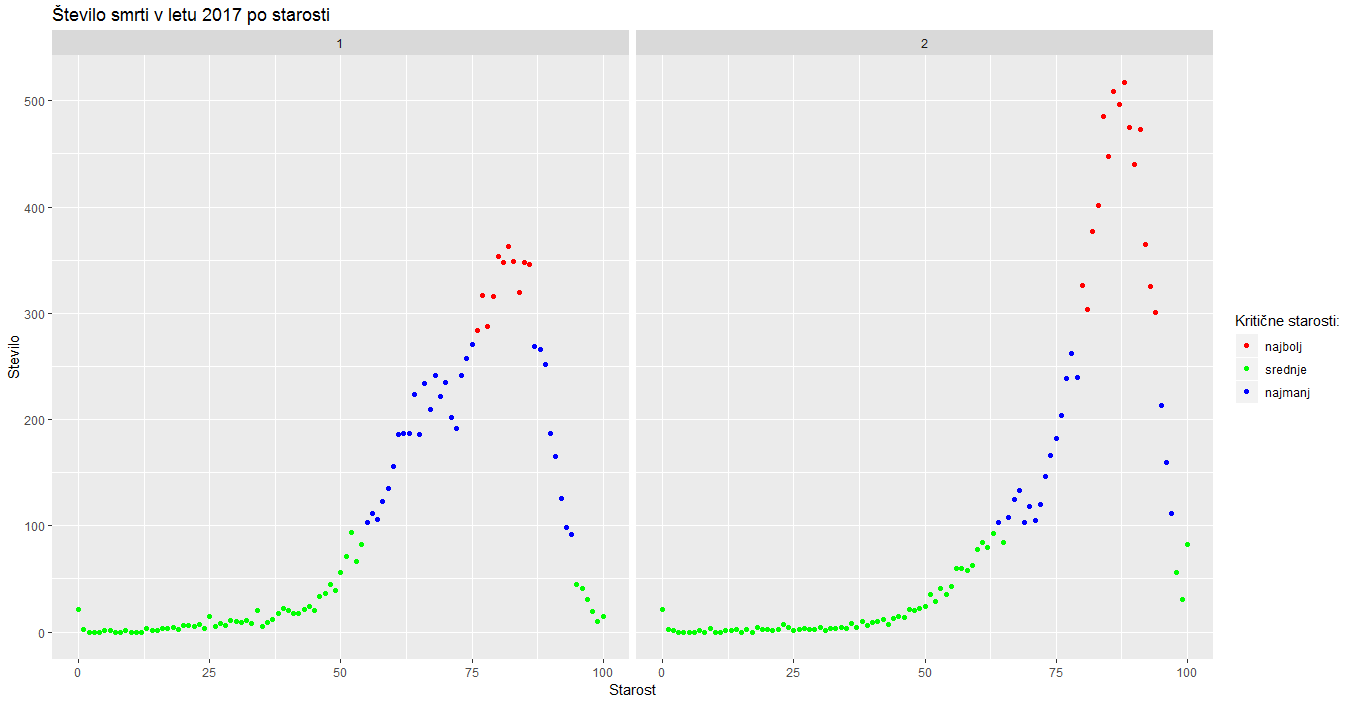
\includegraphics[width=12cm, height=6cm]{grafMNKumrli}
\end{figure}


\noindent Glede na dane rezultate, ki jih vrne \textsl{k}-means algoritem, lahko vidimo, da nam je večino podatkov pogrupiral v skladu s pričakovano krivuljo umrljivosti po starosti. 
Na grafu najbolj kritično starost predstavlja rdeča barva. To so moški med 76 in 86 letom ter ženske med leti 80 in 94. Rezultat ni presenetljiv, saj imajo ženske daljšo življenjsko dobo, kar prikazuje tudi najvišja višina pikic bolj desno na grafu 2.
\noindent Z algoritmom pa sva najmanj optimalno dobila množico $S_2$ (zelena barva). Le-ta vsebuje tako novorojenčke kot tudi visoke starostnike. Ker je tu razpon med leti največji, je tudi vsota razdalj do centra največja. \\

\noindent Prav tako pa sva tudi za ta primer naredil Voronojev diagram, ki nama je razdelil območje na 3 dele.

\vspace{0.5 cm}

\noindent Na koncu sva na tem primeru z Elbowo metodo sprogramirala iskanje oprimalnega $k$ in dobila naslednji graf.

\begin{figure}[h]
\caption{Optimalen $k$}
\centering
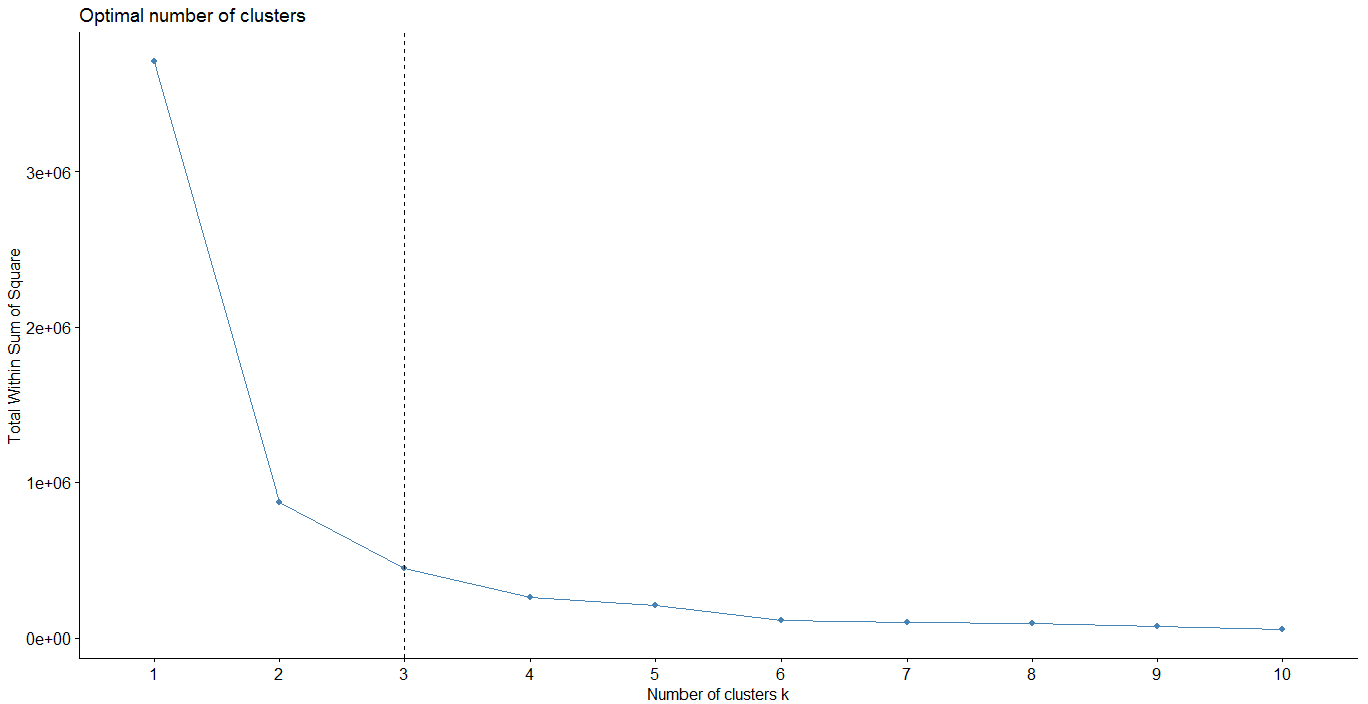
\includegraphics[width=12cm, height=6cm]{optkumrli}
\end{figure}


\newpage

\section{PODATKI V PROSTORU $\mathbb{R}^3$}
\textbf{CILJ:} Poskušala sva pogrupirati avtomobile v skupine na podlagi izbranih karakteristik. \\

\noindent Podatke sva uvozila s pomočjo že vgrajene tabele mtcars.\\
\noindent Na podlagi dobljenih rezultatov se lahko bralec odloči, katere znamke avtomobilov mu bolj ustrezajo, glede na preučevane karakteristike. \\

\vspace{0.5 cm}

\noindent \textbf{PODATKI:} \\
\noindent Za vsak avtomobil so naju zanimali podatki glede na 3 karakteristike: \\
\begin{itemize}
	\item število prevoženih kilometrov z enim galonom goriva;
	\item število konjskih moči;
	\item najmanjši izmerjeni čas na četrtino milje.
\end{itemize}

\noindent Glede na formalno definicijo \textsl{k}-means algoritma so podatki: \\
\begin{itemize}
	\item $ x_1,…,x_{32}$, kjer $x_i$ prikazuje posamezen model avtomobila, \\
	\item $\forall x_i  (i = 1,\ldots, 32)$ je 3-dimanzionalni vektor $\Rightarrow$ za vsak avto so naju zanimale 3 (prej navedene) karakteristike \\
\end{itemize}
S \textsl{k}-means algoritmom sva napravila particijo 32 meritev v 4 množice, \\ 
$ S = \{S_1, \ldots, S_4\}$.  Množice nisva poimenovala, ampak samo različno obarvala (zelena, modra, rumena, vijolična). \\

\noindent \textbf{REZULTATI:} \\
\noindent Rezultati so bili podani v štirih različnih množicah.  \\
\noindent Množica $S_1$, ki je zelene barve, predstavlja znamke avtomobilov z najmanjšo porabo, vendar zato tudi majhno število konjskih moči in pa posledično daljši čas na četrtino milje. \\
\noindent Množica $S_2$, obarvana z modro, predstavlja optimalne izbire avtomobilskih znamk za vsakdanje voznike. Gre za tipe avtomobilov, ki lahko prevozijo do 30 milj z eno galono goriva, prav tako pa imajo zadosti konjskih moči (čez 100 hp) in sorazmerno nizek čas za prevoz četrtine milje (17 sekund). \\
\noindent V tretji množici $S_3$, obarvani z rumeno, imajo podatki najmanjšo vsoto razdalj do njihovega centra (najbolj prilegajoči se podatki centru). Le-ta vsebuje avtomobilske znamke, ki imajo dokaj podobno porabo, kot avtomobili iz zadnje množice (vijolično obarvani). Vendar imajo avti v $S_3$ precej manj konjskih moči in daljši čas za prevoz četrtine milje. \\
\noindent Tako bi se kot kupec s stališča porabe, pri izbiri med množicama $S_3$ in $S_4$, raje odločil za nakup avtomobila iz množice $S_4$.

\newpage

\section{VIRI}
\noindent L. Kaufman, P. J. Rousseeuw, \textsl{Finding groups in data: An introduction to cluster analysis}, John
Wiley Sons, Chichester, UK, 2005. 

\vspace{0.5cm}

\noindent  J. Kogan, \textsl{Introduction to Clustering Large and High-dimensional Data}, Cambridge University
Press, New York, 2007.



\end{document}